\section{Culture conditions, strains and worm handling}\label{sec:wormHandling}
\acs{ce} worms were cultured on \ac{ngm} agar plates seeded with OP50 \ac{ecoli} (a slow-growing \ac{ecoli} bacterial strain), and handled as described in \cite{brenner1974genetics}. Worms were maintained at \SI{20}{\celsius}. The following strains were used in this work:

\begin{table}[h!]
    \centering
    \begin{tabular}{| c | c | m{0.4\textwidth} |} 
        \hline
        Strain & Fluorescent tags & \hfil Genotype \\
        \hline
        SWG070 & NMY-2::GFP, PH-Domain::mCherry & nmy-2(cp7[nmy-2::gfp + LoxP unc-119(+) LoxP]) I; ltIs44 [pAA173 pie-1p-mCherry::PH(PLC1delta1) + unc-119(+)]\\[3em]
        SWG057 & TUB::GFP, NMY-2::mKate & nmy-2(cp7[nmy-2::gfp + LoxP unc-119(+) LoxP]) I; ltIs44 [pAA173 pie-1p-mCherry::PH(PLC1delta1) + unc-119(+)]\\[3em]
        SWG228 & NMY-2::GFP & nop-1 mutant\\[3em]
        CB207 & --- & dpy-11 mutant\\[3em]
        SWG297 & NMY-2::GFP, PH-Domain::mCherry & cross between CB207 and SWG070\\
        \hline
    \end{tabular}
    \caption{\ac{ce} strains used in this study}
    \label{tab:ceStrains}
\end{table}

The primary strain used in this work is a dual-color strain labelled with \acs{nmy2}::\acs{gfp} and phDomain::mCherry, named SWG070. This transgenic strain labels \ac{nmy2} myosin with \acf{gfp} and PH domain (localized to the cell membrane \citep{park2008comprehensive}) with mCherry (a red fluorescent protein \citep{shaner2004improved}). Thus, SWG070 enable visualization of the myosin distributions in the embryo and its cell membrane during its development.

For experiments with \textit{goa-1}; \textit{gpa-16} double \ac{rnai}, SWG057 was used. This strain labels tubulin with \ac{gfp} and \ac{nmy2} myosin with mCherry. This allows visualization of the centrosomes in this condition, required for evaluating if the \ac{rnai} was successful. 

\section{Genetic perturbations by \acs{rnai}}\label{sec:rnaiMethods}
In order to achieve specific effects (example: embryos deficient in pseudocleavage furrow), we reduced expression of specific genes via \acl{rnai} (example: NOP-1). All \acf{rnai} experiments were performed via feeding, as previously described \citep{timmons2001ingestion,kamath2003genome}. For this process, \ac{rnai} feeding plates were generated by seeding \ac{ngm} agar plates, containing \SI{1}{\milli\Molar} isopropyl-$\beta$-D-thiogalactoside and \SI{50}{\micro\gram\per\milli\liter} ampicillin, with the bacterial expressing the \ac{dsRNA} targeting the gene of interest, and grown overnight. \ac{rnai} was then performed by transferring young L4 worms onto these \ac{rnai} feeding plates and incubating them for the specified time at \SI{20}{\celsius} before imaging. See \autoref{tab:RNAiTime} for incubation times used. For single \ac{rnai} interference experiments, only the \ac{rnai} clone of interest was grown on the \ac{rnai} feeding plates. For double \ac{rnai} interference of \textit{nop-1} and \textit{mel-11}, both \ac{rnai} clones were grown simultaneously on the \ac{rnai} feeding plates. For double \ac{rnai} interference of \textit{goa-1} and \textit{gpa-16}, sequences targeting both genes were integrated into a single bacterial clone, which was grown on the feeding plates.

\begin{table}[h]
    \centering
    \begin{tabular}{| c | c |} 
        \hline
        \ac{rnai} condition & Feeding time\\
        \hline
        \textit{mlc-4} & \SIrange{22}{24}{\unitRNAiTime}\\ 
        \textit{nop-1} & \SIrange{24}{27}{\unitRNAiTime}\\
        \textit{nop-1}; \textit{mel-11} (double) & \SIrange{24}{27}{\unitRNAiTime}\\
        \textit{ima-3} & \SIrange{20}{24}{\unitRNAiTime}\\
        \textit{air-1} & \SIrange{24}{27}{\unitRNAiTime}\\
        \textit{goa-1}; \textit{gpa-16} (double) & \SIrange{24}{27}{\unitRNAiTime}\\
        \hline
    \end{tabular}
    \caption{Feeding times for \acs{rnai} conditions}
    \label{tab:RNAiTime}
\end{table}

All bacterial clones, except from \textit{mlc-4} and \textit{goa-1}; \textit{gpa-16} double \ac{rnai} clone, were obtained from the Ahringer RNAi library (Source Bioscience) \citep{kamath2003genome}. The \textit{mlc-4} \ac{rnai} clone was obtained from the Hyman lab. The \textit{goa-1}; \textit{gpa-16} double \ac{rnai} clone was obtained from the Kotak lab.

\section{Time-lapse microscopy}\label{sec:microscope}
All movies of \ac{ce} embryos were obtained at room temperature, using a spinning-disk confocal microscope with Zeiss Axio Observer Z1 equipped with Yokogawa CSU-X1 scan head, a C-Apochromat 63X/1.2 NA Water objective, a Hamamatsu ORCA-Flash4.0 V2 CMOS camera (\SI{2048}{\pixels} by \SI{2048}{\pixels}, pixel size of \SI{0.105}{\micro\meter}), and operated using Micro-Manager \citep{edelstein2014advanced}. The microscope is equipped with \SI{488}{\nano\meter} and \SI{561}{\nano\meter} solid-state imaging lasers.

To prepare a sample for imaging, adult worms (typically \num{2} per drop) were picked from agar plates and transferred in a drop (vol: \SI{7}{\micro\liter}) of M9 buffer (\SI{22}{\milli\Molar} \ce{KH2PO4}, \SI{42}{\milli\Molar} \ce{Na2HPO4}, \SI{86}{\milli\Molar} \ce{NaCl}) placed on a cover slip. \SI{20}{\unitLength} polystyrene beads were added to the M9 buffer to act as spacers for imaging -- ensuring the height of embryo after mounting is atleast \SI{20}{\unitLength}. To obtain one-cell stage embryos, these worms were dissected using a syringe tip to extract the embryos from the worm body into the M9 buffer. 

The M9 droplet with embryos was mounted on a microscope slide, and transferred to the microscope. The sample is scanned using a \num{10}X objective with transmitted light to find one-cell embryos before onset of \ac{ap} axis establishment. Such embryos can be recognized by the smooth cytoplasm and lightly ruffled cell membrane. Once an embryo has been identified for imaging, the objective is changed to the \num{63}X water objective. The focus is brought to the midplane of the embryo, and the image acquisition process is started.

3-channel time-lapse movies were acquired by taking three images at each time-point: one using transmitted light (denoted here as \ac{bf}), one using \SI{488}{\nano\meter} excitation laser (for imaging \ac{nmy2}::\ac{gfp}) and one using \SI{561}{\nano\meter} excitation laser (for imaging cell membrane) -- see \autoref{subfig:imageAcquisition-swg070}. All images are taken at the midplane of the imaged embryo. Movies were acquired at \SI{3}{\second} intervals between time-points, with \SI{50}{\milli\second} exposure time for transmitted light, \SI{200}{\milli\second} exposure time for \ac{gfp} and \SI{150}{\milli\second} exposure time for mCherry. Embryos were imaged starting from the onset of cortical flows until pronuclear meeting. $T =$ \SI{0}{\second} was selected at the end of posteriorization of the male pronucleus; that is, the time-point after which the male pronucleus moves away from the cortex and towards the female pronucleus. All movies were synchronized using this time-point.

For SWG057, a slight variation of the above process was followed  -- see \autoref{subfig:imageAcquisition-swg057}. At each time-point, a \ac{bf} image using transmitted light and a \ac{nmy2} image using \SI{561}{\nano\meter} excitation laser were taken at the midplane of the embryo. Additionally, a z-stack of \num{11} slices, with uniform spacing of \SI{1}{\micro\meter}, was taken using the \SI{488}{\nano\meter} excitation laser. This z-stack is used later to facilitate detection of embryo boundary. Movies were acquired at \SI{5}{\second} intervals between time-points, with \SI{50}{\milli\second} exposure time for transmitted light, \SI{100}{\milli\second} exposure time for each slice of the z-stack in \ac{gfp} and \SI{150}{\milli\second} exposure time for mKate.

\begin{figure}[h]
\centering
\begin{subfigure}{\textwidth}
    \centering
    \includegraphics[width=\textwidth]{ExpMethods/FigChannelImages/swg70.pdf}
    \caption{Microscope images of an embryo of SWG070 strain acquired during time-lapse microscopy, depicting the three channels recorded. Top: Bright field, Middle: \ac{nmy2}::\ac{gfp} (myosin), Bottom: phDomain::mCherry (boundary). The male pronucleus can be visualized as the dark circle in the myosin channel towards the posterior end (right). T = \SI{0}{\second} is set at the end of posteriorisation. Scale bar: \SI{10}{\unitLength}} 
    \label{subfig:imageAcquisition-swg070}
\end{subfigure}
\hfill
\begin{subfigure}{\textwidth}
    \centering
    \includegraphics[width=\textwidth]{ExpMethods/FigChannelImages/swg57.pdf}
    \caption{Microscope images of an embryo of SWG057 strain acquired during time-lapse microscopy, depicting the three channels recorded. Top: Bright field, Middle: \ac{nmy2}::mKate (myosin), Bottom: tub::\ac{gfp} (microtubules - we will extract the boundary from this). The male pronucleus can be visualized as the dark circle in the myosin channel towards the posterior end (right). For microtubule channel, the max projection of the z-stack is shown (see \autoref{fig:preprocessSWG057} for example of full z-stack). T = \SI{0}{\second} is set at the end of posteriorisation. Scale bar: \SI{10}{\unitLength}} 
    \label{subfig:imageAcquisition-swg057}
\end{subfigure}
\caption[Image acquisition]{Image acquisition during time-lapse microscopy for SWG070 and SWG057 strain. Images are rotated such that anterior and posterior ends are to the left and right respectively.}
\label{fig:imageAcquisition}
\end{figure}

\section{Image analysis}\label{sec:imageAnalysis}
In this section, we describe the general image analysis pipeline that was used to analyse the movies that were acquired from the microscope. We will mainly focus on movies generated using the SWG070 strain, which will be the primary strain used in this work. However, the analysis pipeline itself can be used for movies from other strains, after certain modifications if needed. For SWG297, since the fluorescent tags are the same, the analysis pipeline can be used without modifications. For SWG057, the pre-processing stage is modified -- which we describe below. Any specific details regarding the analysis of movies generated for a given experiment will be described in the respective sections in \autoref{ch:Results}.

The image analysis pipeline presented here is modified from image analysis pipelines from M. Kramer \citep{mirna2015linking} and P. Gross \citep{gross2019guiding}. The following softwares were used in the image analysis pipeline: \ac{fiji} \citep{schindelin2012fiji,linkert2010metadata} for pre-processing, Python \citep{python38} for tracking the male pronucleus and setting up the inputs for measurements of cortical flows, and \ac{matlab} \citep{MATLAB:2016a} for measurement of cortical and cytoplasmic flows using \acs{piv} and constructing averages of various quantities over the ensemble of embryos in each condition. A custom PowerShell script was used for automated batch processing of movies.

\subsection{Pre-processing}\label{subsec:preprocess}
Movies are pre-processed using a custom \ac{fiji} macro. For each movie, the following steps are performed in order:
\begin{enumerate}
    \item Each movie is cropped to ensure that only a single embryo is present in each frame. If other embryos are present in the cropped frame, they are cleared to black using the \emph{Clear...} command in \ac{fiji}.
    \item Anterior and posterior end of the embryo of interest are manually selected. Posterior side is identified by the depletion of \ac{nmy2} on the posterior end of the cortex. The movie is rotated using bi-linear interpolation such that the anterior and posterior ends of the embryo of interest are on the left and right sides of the frame respectively (see \autoref{subfig:preprocess-manual}).
    \item The pronuclei can be seen as grey circles in the \ac{bf} and dark circles in the \ac{nmy2} channels, located in the cytoplasm. The male pronucleus is identified as the pronucleus towards the posterior end. The movie is flipped to ensure that the male pronucleus is located near the top side of the frame at the start of posteriorization. Any movies with both pronuclei on the same side are discarded  (see \autoref{subfig:preprocess-manual}).
    \item The first frame in the movie at which the male pronucleus appears and the last frame before the male pronucleus moves away from the cortex were manually selected. Only frames between these two selected frames will be analysed  (see \autoref{subfig:preprocess-selectNucleusRange}).
\end{enumerate}

\begin{figure}[h]
\centering
\begin{subfigure}{\textwidth}
    \centering
    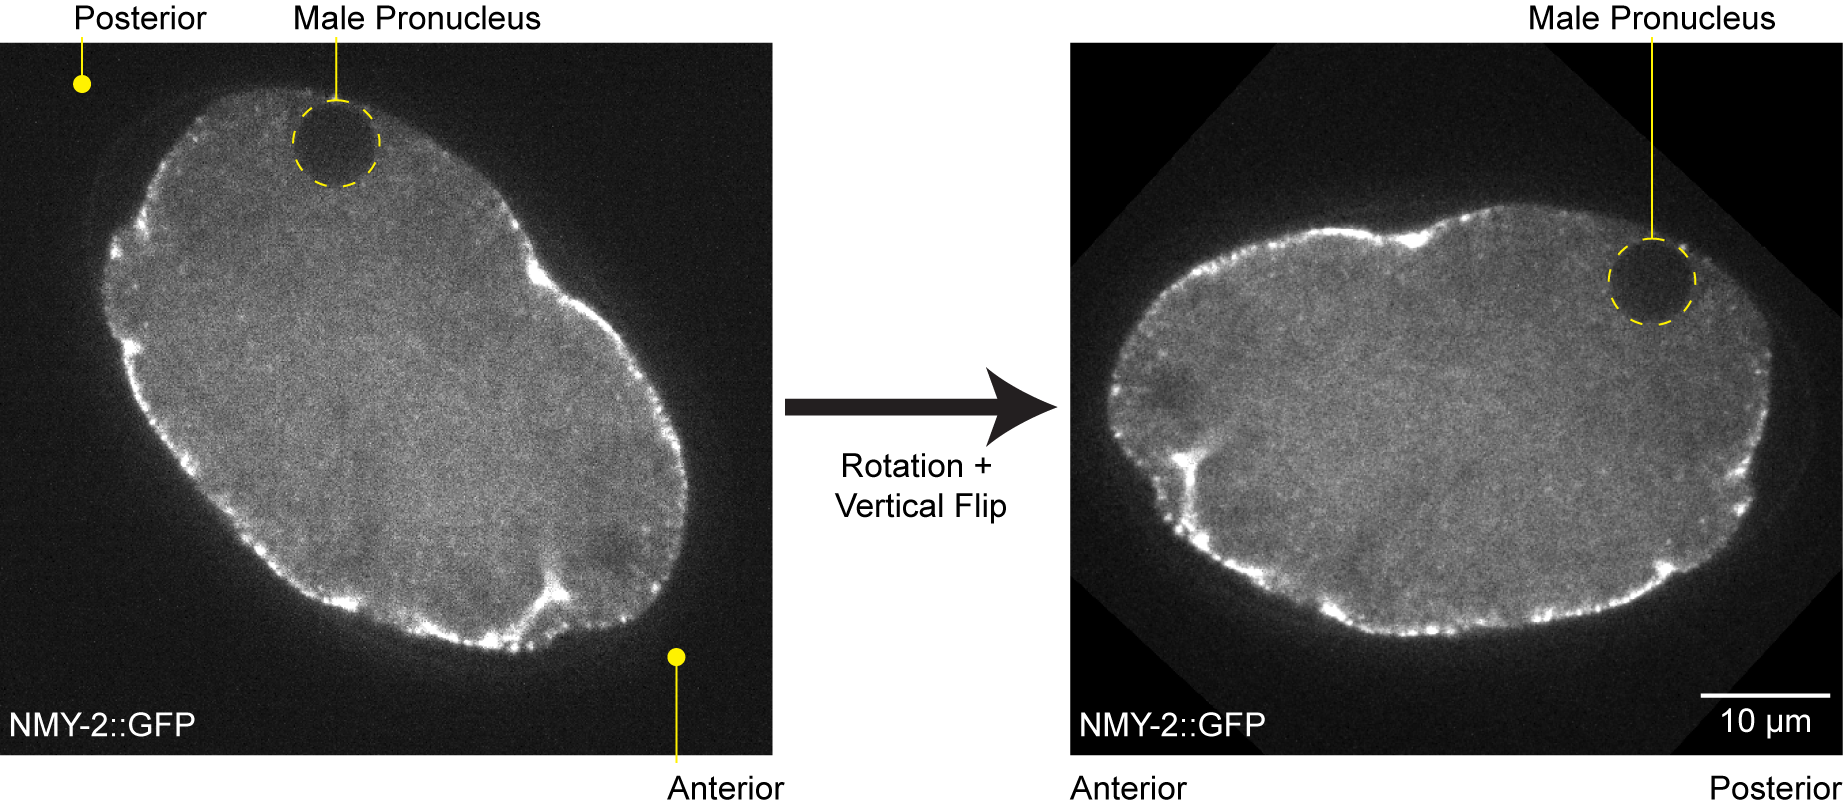
\includegraphics[width=0.9\textwidth]{ExpMethods/FigPreProcess/manualAnnotationRotation.png}   \caption{Left image (myosin channel) demonstrates the manual annotation done during pre-processing. Posterior end is recognized by the the presence of the male pronucleus (yellow dotted circle) and the associated depletion of myosin on the cortex. Two points are then marked to denote the posterior and anterior ends respectively (yellow dots near the ends of the embryo). Right image shows the result -- the image is rotated and then flipped (if necessary) to ensure that the anterior and posterior ends are on the left and right of the frame, and that the male pronucleus moves from the top of the embryo towards the posterior end. Scale bar: \SI{10}{\unitLength}} 
    \label{subfig:preprocess-manual}
\end{subfigure}
\hfill
\begin{subfigure}{\textwidth}
    \centering
    \includegraphics[width=\textwidth]{ExpMethods/FigPreProcess/selectNucleusRange.pdf}
    \caption{Myosin frames at different time-points depicting the movement of the male pronucleus (after rotation and flip). The frame where the male pronucleus first appears is denoted as the first frame. The frame where the male pronucleus starts moving away from the cortex -- and therefore the frame where posteriorisation ends -- is denoted as the last frame. Only the time-points that lie between the first and last frame are analysed (indicated by yellow dotted line). Time-points are denoted in \unit{\second}, with T = \SI{0}{\second} selected as the last frame, i.e. end of posteriorisation. Scale bar: \SI{10}{\unitLength}} 
    \label{subfig:preprocess-selectNucleusRange}
\end{subfigure}
\caption[Image analysis: pre-processing]{Pre-processing steps in the image analysis pipeline, for SWG070 strain. Anterior and posterior are to left and right respectively in all images.}
\label{fig:preprocess}
\end{figure}

For movies generated using SWG057 strain, step 1 of the pre-processing is modified --  see \autoref{fig:preprocessSWG057}. z-stack collected in the \ac{gfp} channel is used to detect the boundary of the embryo of interest in the frame. Kuwahara filter with window size \num{11} is used for noise reduction while still preserving edges \citep{kuwahara1976processing}. The z-stack is thresholded using the default thresholding method used by \ac{fiji} \citep{imageJGuide}. Maximum projection of this binary stack is then used to generate embryo boundary. If multiple embryos are present, only the binary mask corresponding to the embryo of interest is retained. The \ac{bf} images, \ac{nmy2} images and embryo outlines are arranged together in the same channel arrangement as those used for SWG070 movies. After this modification, movies from SWG057 strain are processed in the same as movies from the SWG070 strain.

\begin{figure}[h]
\centering
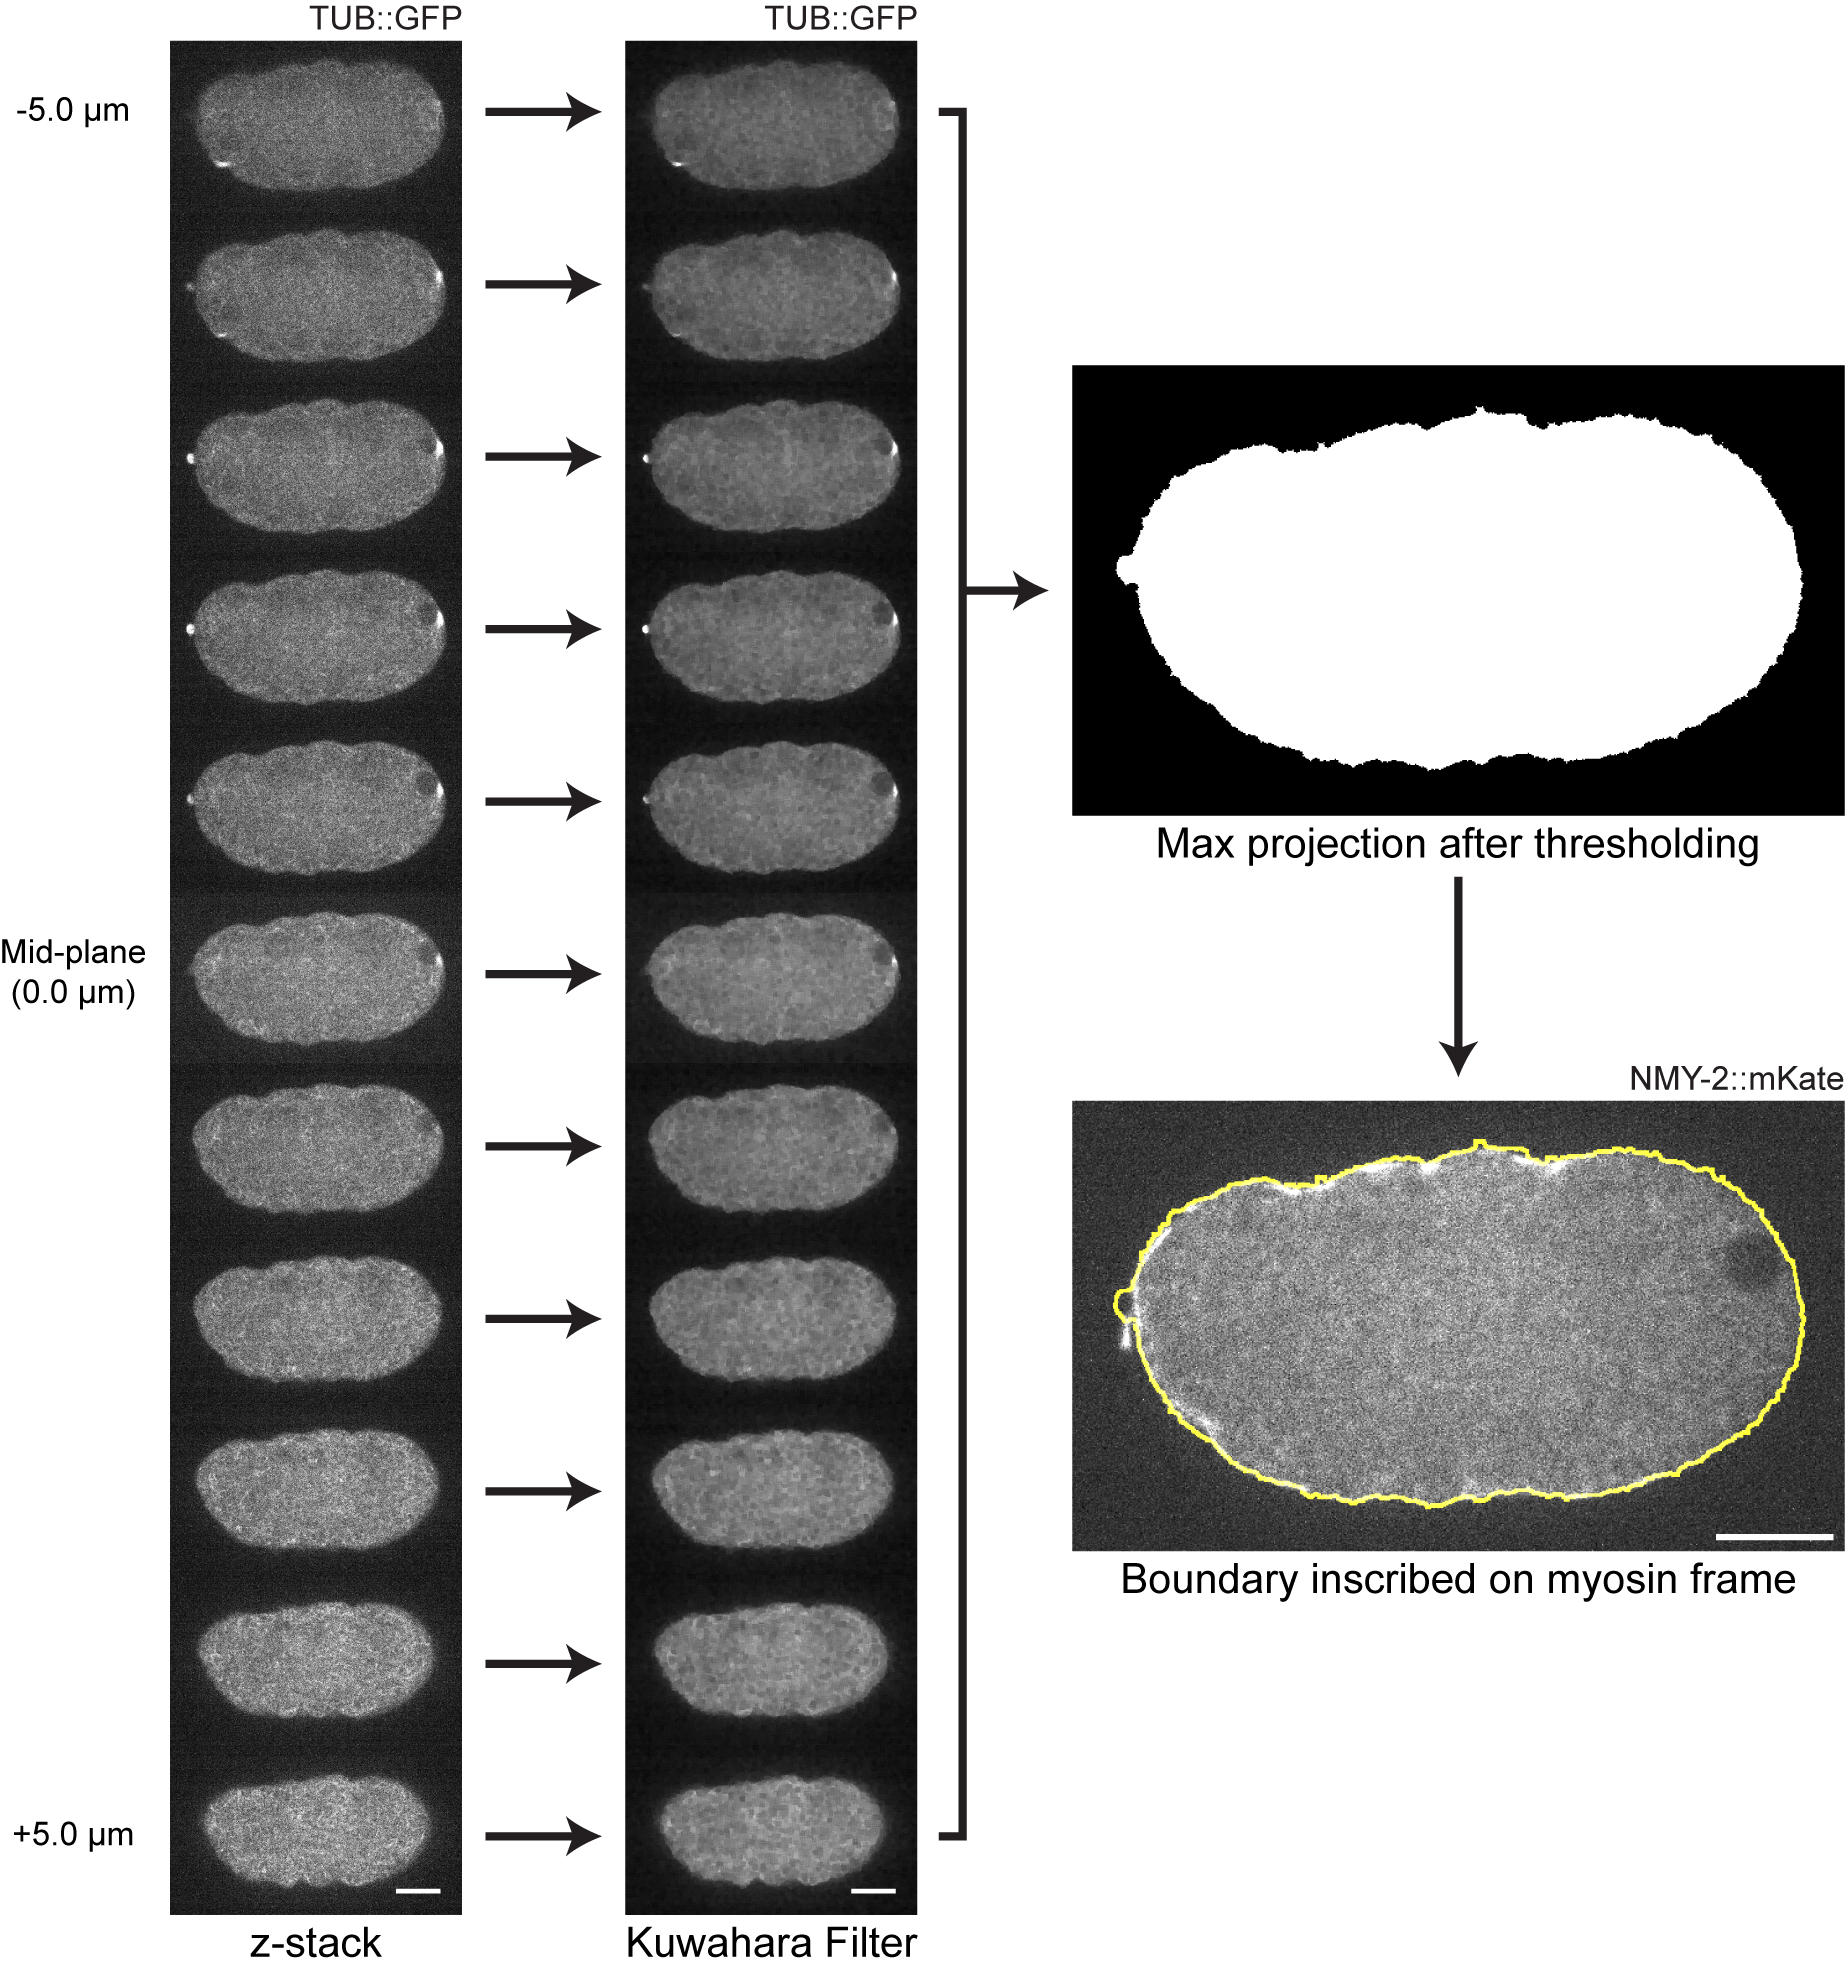
\includegraphics[width=\textwidth]{ExpMethods/FigPreProcess/swg057BoundaryDetect.png}
\caption[Image analysis: pre-processing (SWG057)]{Modified pre-processing steps for SWG057 strain, to extract embryo boundary from microtubule z-stacks. At each time-point, the z-stack of \num{11} slices in the microtubule channel are filtered using the kuwahara filter, binarized and then max projected. The outline of the max projection is encoded as the boundary channel, mimicking the phDomain::mCherry channel of the SWG070 strain. This outline is shown here as the yellow boundary inscribed onto the myosin frame at the same time-point. Scale bars in all images: \SI{10}{\unitLength}. Anterior and posterior are to left and right respectively in all images.}
\label{fig:preprocessSWG057}
\end{figure}

\subsection{Tracking posteriorisation of the male pronucleus}\label{subsec:nucleusTracking}
To track the position of the male pronucleus as it posteriorises, processed movies were analysed using a custom Python script. Following external packages were used in this Python script: openCV \citep{opencv}, tifffile \citep{tifffile}, scipy \citep{scipy} and numpy \citep{numpy}. This script expects the input movies to be a multipage tiff file with three channels -- first for \ac{bf} (which is not used in analysis), second for \ac{nmy2} and third denoting embryo boundary (example -- phDomain::mCherry in SWG070). We will refer to them as the \ac{bf} channel, the myosin channel, and the boundary channel respectively.

\subsubsection{Segmenting the embryo boundary}\label{subsubsec:boundaryDetect}
For each time-point, the boundary channel frames are extracted and smoothed using a gaussian filter (with sigma = \SI{2}{\pixels}). Each frame are then thresholded using the 90th percentile of the intensity values in that frame as the threshold. A morphological closing operation (with disk element of size \SI{17}{\pixels}) is performed on the binary image thus constructed, to close any gaps in the boundary. To detect if the segmented embryo boundary is indeed closed, the inside of the boundary is filled using a binary fill holes operation. If the boundary is not filled, this operation will fill the whole frame instead. Thus, to detect if the boundary was closed, we check if more than \num{80}\% of the frame is filled. If less than \num{80}\% of the frame was filled, the boundary is closed -- which we segment as the contour of non-zero length enclosing the largest area in the frame. If more than \num{80}\% of the frame was filled, we dilate (with disk element of size \SI{18}{\pixels}) the binary frame with the segmented boundary to attempt closing gaps again. If after the dilation, binary fill holes still leads to more than \num{80}\% of the frame being filled, we consider the boundary detection to be failed for this time-point and use the boundary segmented in the previous time-point. Otherwise, the contour of non-zero length enclosing the largest area in the frame after dilation is again considered as the boundary. Boundary segmented at the previous time-point is also used if the boundary segmented at the current frame has a length too different from the previous one.

For each time-point, the segmented boundary is fit to an ellipse and the long and short axes of the fitted ellipse are calculated. To obtain the average axes for the movie, the axes detected for each time-point are averaged. The average direction is found by averaging the unit vectors that denote the instantaneous directions of the axes in each time-point, and the average lengths by averaging the lengths of the instantaneous axes. See \autoref{fig:segmentingEmbryoBoundary} for an example.

Additionally, the myosin channel frames are also denoised using non-local means denoising \citep{buades2011non}, with the following parameters: Filter strength = \SI{3}{\pixels}, template window size = \SI{4}{\pixels}, search window size = \SI{12}{\pixels}. 

\begin{figure}[h]
\centering
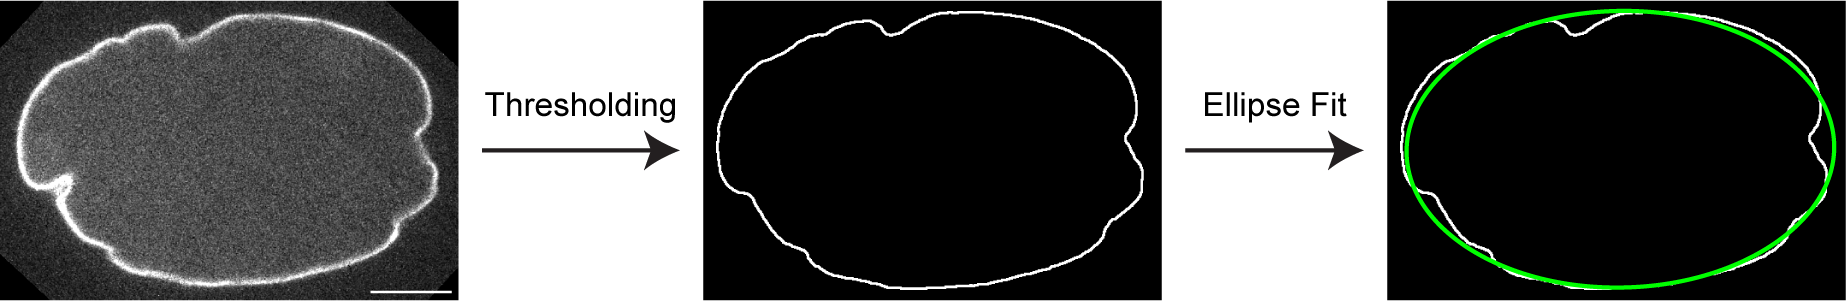
\includegraphics[width=\textwidth]{ExpMethods/FigTrackingPipeline/boundaryDetect.png}
\caption[Image analysis: Segmenting embryo boundary]{Boundary detection using the phDomain::mCherry channel in SWG070. At each time-point, the frame (left) is thresholded (middle, see \nameref{subsubsec:boundaryDetect} for details). The thresholded image provides the segmented boundary. An ellipse is fit to this segmented boundary to obtain the instantenous long and short axes (right, yellow line indicates the fitted ellipse). The same process is carried out on movies generated using embryos from the SWG057 strain. Scale bar: \SI{10}{\unitLength}}
\label{fig:segmentingEmbryoBoundary}
\end{figure}

\subsubsection{Segmenting the male pronucleus}\label{subsubsec:nucleusDetect}
The denoised myosin channel frames are utilized for segmenting the male pronucleus. We only consider myosin frames for the time-points in the range selected in \autoref{subsec:preprocess}. In these frames, the pronuclei can be identified as dark circles devoid of myosin in the cytoplasm. The male pronucleus is identified as the one present in the posterior half (steps in \autoref{subsec:preprocess} ensure we always have this). We utilize this difference in intensities between the cytoplasmic myosin and male pronucleus to segment the latter, using successive thresholding. The following steps are undertaken for each myosin frame (that is, at each time-point) to segment the male pronucleus (see \autoref{fig:malePronucleusTrackingPipeline} for an example):
\begin{enumerate}
    \item The segmented embryo boundary is used to create a mask of the interior of the embryo -- in this way, the boundary segmentation is crucial for male pronucleus segmentation, as it allows separating the interior of the embryo from the whole frame.
    \item The set of thresholds to use for successive thresholding is selected, ranging from the \num{5}th to the \num{95}th percentile of the non-zero intensity values in the embryo interior.
    \item For each threshold in the selected range:
    \begin{enumerate}
        \item The frame is thresholded using the selected threshold. Pixels with intensity values below the selected threshold are set to be white (= \num{1}), and rest to black (= \num{0}).
        \item All pixels to the left (or in the anterior half) of the embryo center (determined as the center of the ellipse fit to the boundary) are set to black (= \num{0}). This ensures that we detect only the male pronucleus, which is present to the right (or in the posterior half). A morphological opening operation with disk element of size \SI{5}{\pixels} is performed to remove small regions of white pixels.
        \item The total number of white pixels for this threshold is recorded.
    \end{enumerate}
    \item To detect the thresholds to use for male pronucleus segmentation, the \enquote{knee} of the Number of white pixels vs Thresholds graph is detected. This \enquote{knee} indicates the threshold above which which the number of white pixels for each threshold increase rapidly, indicating that the white pixels are \enquote{flooding} outside the dark circle that denotes the male pronucleus. To detect this \enquote{knee}, at each threshold we calculate a cost function: the square root of the average of differences from the mean of the number of white pixels up until that threshold is calculated. The threshold for which this cost is the lowest is selected as the maximum threshold to be used for male pronucleus segmentation. See \autoref{subfig:malePronucleusTrackingPipeline-successiveThreshold} for an example.
    \item All thresholds upto this maximum threshold calculated in the last step are considered. The male pronucleus is identified as a dark circle. To quantify how circular a segmentation is, we use the circularity measure\footnote{This measure is based on the isoperimeteric inequality: a geometric inequality that relates the surface area (perimeter for 2D) to the volume (area for 2D) of a region. In 2D, it states that the perimeter of any closed curve $L$ is related to the enclosed area $A$ as $L^2 >= 4\pi A$. Thus, in 2D, for all closed curves with the same perimeter, the one enclosing the most area is the circle.} $ = 4\pi\frac{\textrm{Area}}{\textrm{Perimeter}^2}$, where Area and Perimeter are of the segmented section. Circularity is a dimensionless measure that ranges from \num{0} to \num{1}, with \num{1} being a perfect circle. From all segmentations generated by the thresholds considered in this step, we identify the one that has the largest area and circularity as the male pronucleus. See \autoref{subfig:malePronucleusTrackingPipeline-thresholdSelection} for an example.
\end{enumerate}

\begin{figure}[h]
\centering
\begin{subfigure}{\textwidth}
    \centering
    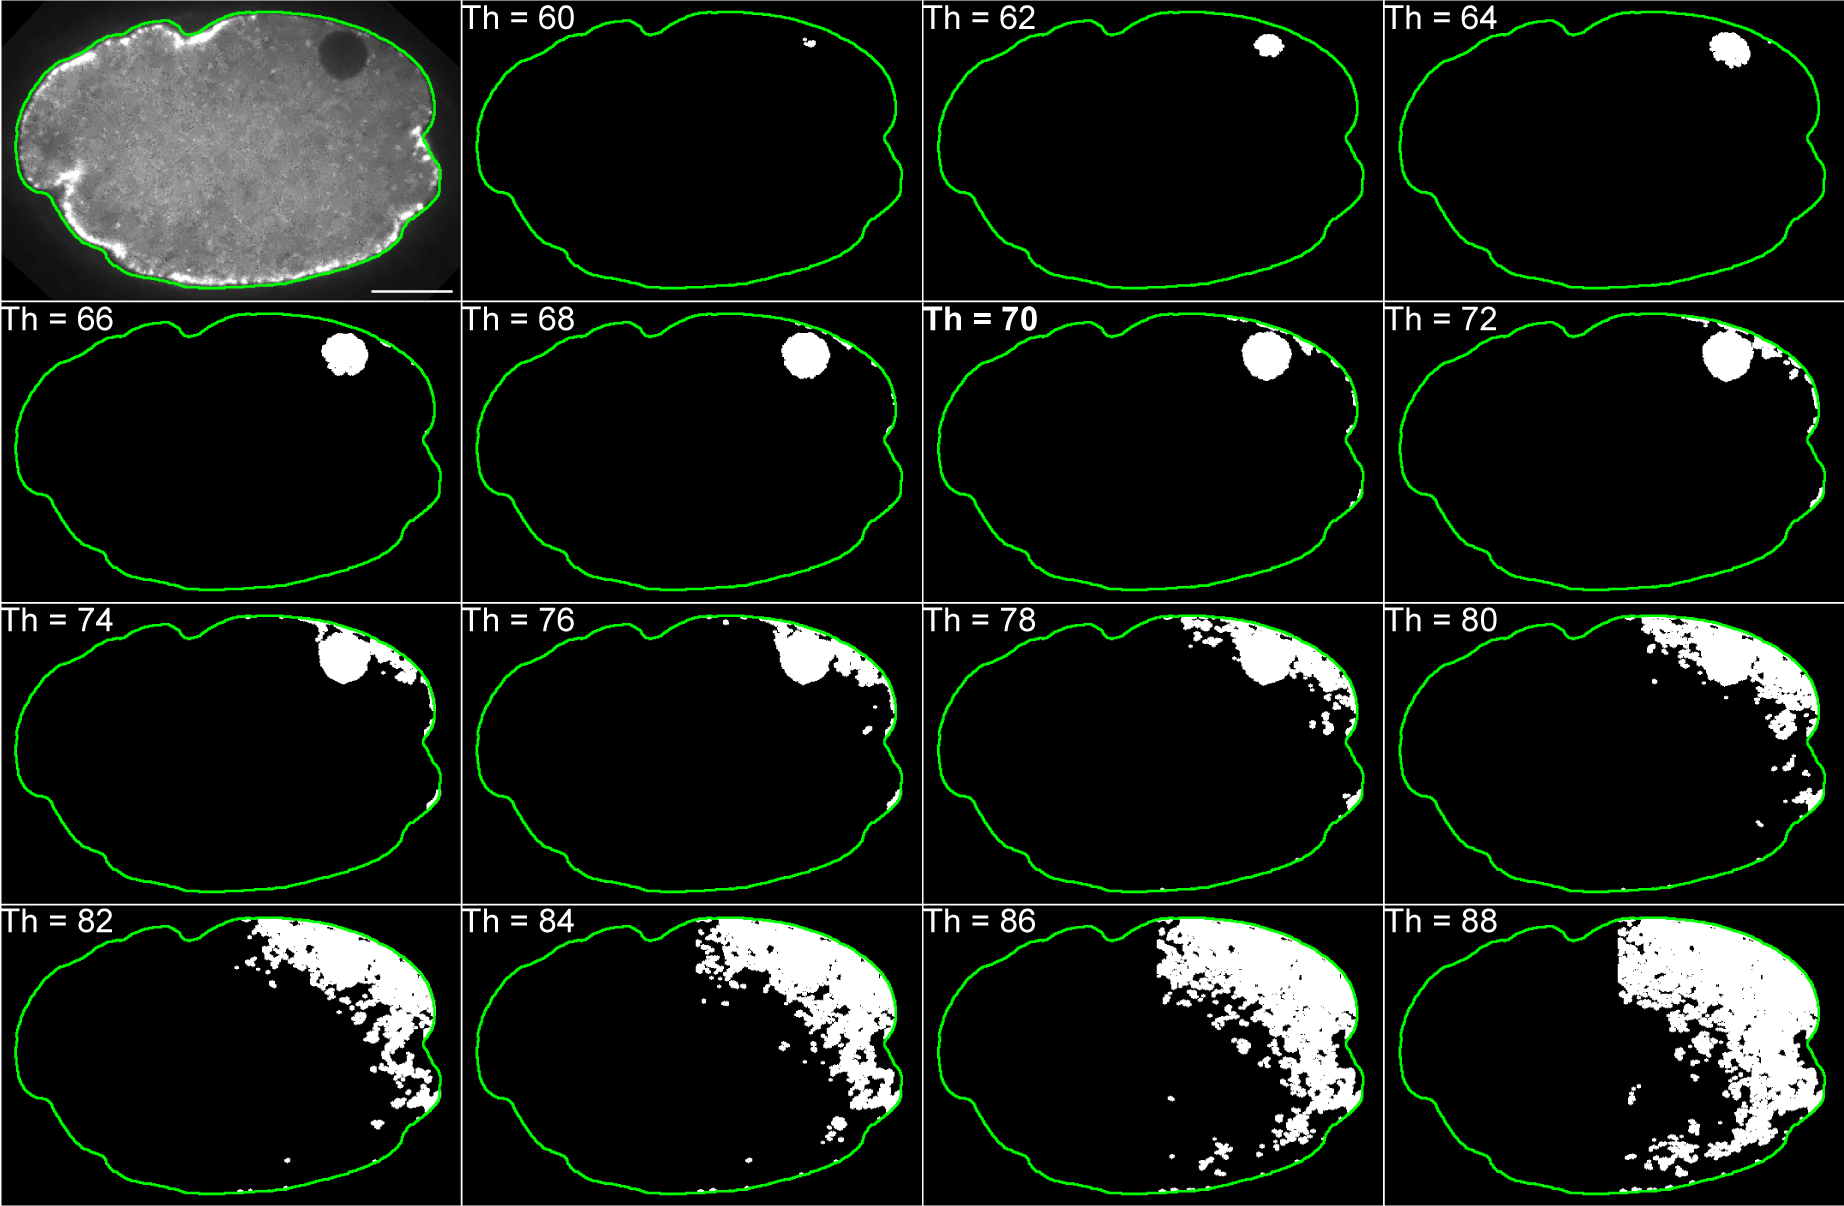
\includegraphics[width=0.9\textwidth]{ExpMethods/FigTrackingPipeline/successiveThreshold.png}
    \caption{Successive thresholding on myosin frame to segment male pronucleus. Top left image is the denoised myosin frame. All pixels outside this contour are ignored for the purposes of thresholding. Rest of the images show the result after thresholding at a specific threshold -- White pixels have intensities below the selected threshold. Yellow contour indicates the segmented boundary for all images. Note that any white pixels in the left half (that is, anterior half) of the embryo are automatically discarded. Threshold = \num{70} is selected for this myosin frame -- see \autoref{subfig:malePronucleusTrackingPipeline-thresholdSelection}. Scale bar: \SI{10}{\unitLength}} 
    \label{subfig:malePronucleusTrackingPipeline-successiveThreshold}
\end{subfigure}
\hfill
\vspace{1mm}
\begin{subfigure}{\textwidth}
    \centering
    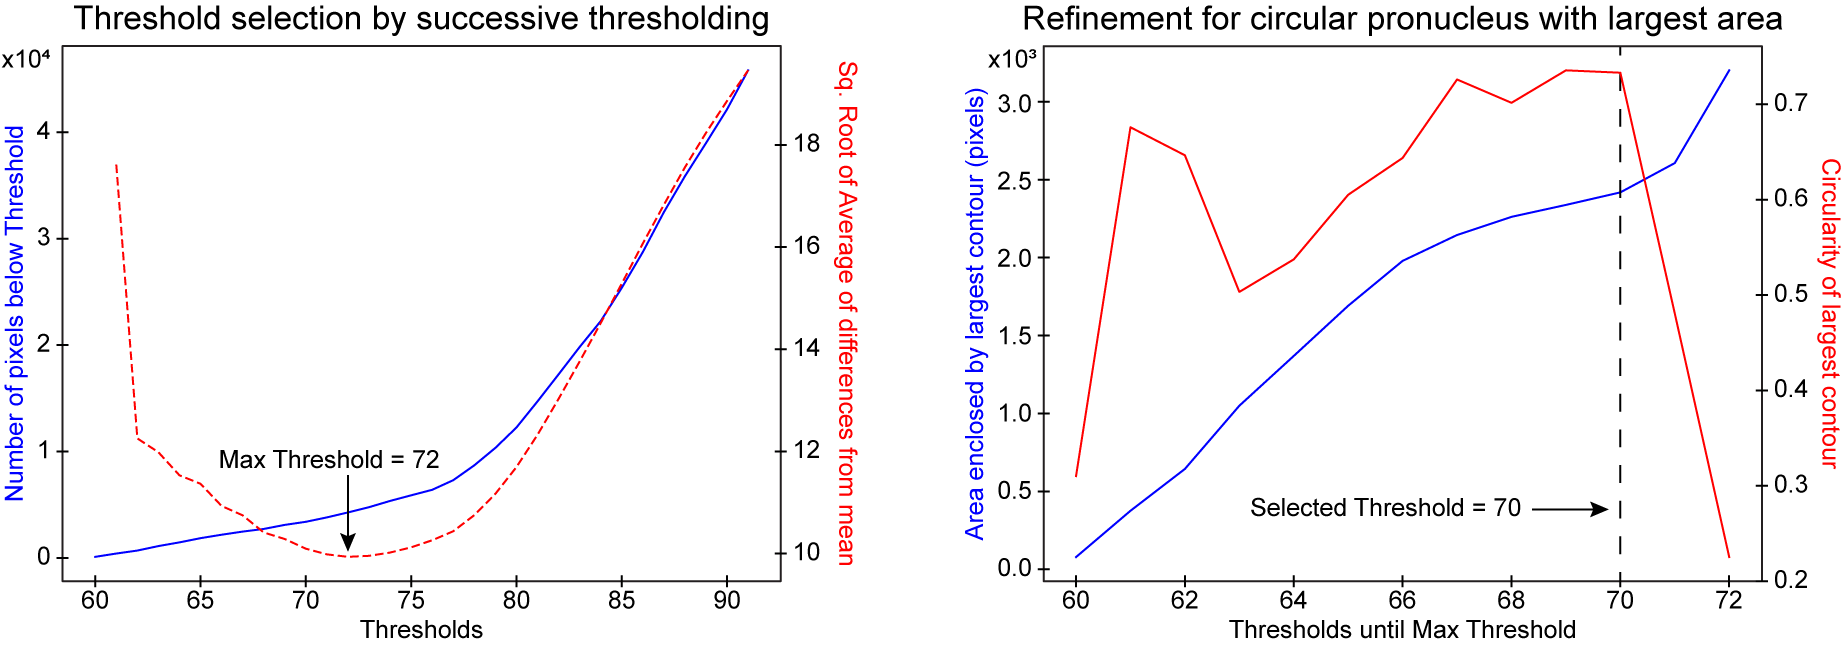
\includegraphics[width=\textwidth]{ExpMethods/FigTrackingPipeline/thresholdSelection.png}
    \caption{Automatic threshold selectiong using successive thresholding (see \nameref{subsubsec:nucleusDetect}). Left: Selecting Max Threshold. Blue curve (left y-axis) depicts the number of white pixels in the sense of \autoref{subfig:malePronucleusTrackingPipeline-successiveThreshold} for each threshold. We want to select Max Threshold near the \enquote{knee} of this curve. Red dotted curve (right y-axis) depicts the cost function. Max Threshold is selected as the threshold with the minimum cost. Right: Selecting Threshold. All thresholds upto Max Threshold are considered. For each threshold, the area of the largest contour (that is, boundary of the largest connected component) is calculated (blue curve, left y-axis). Additionally, the circularity of this contour is calculated (red curve, right y-axis). Final selected threshold for this frame is where the area and circularity are both maximised. For this frame, the selected threshold is \num{70}. See \nameref{subsubsec:nucleusDetect} for definitions} 
    \label{subfig:malePronucleusTrackingPipeline-thresholdSelection}
\end{subfigure}
\caption[Image analysis: Segmenting the male pronucleus]{Segmenting the male pronucleus by successive thresholding and automatic selection. Only a single time-point is considered throughout the figure. Anterior and posterior are to left and right respectively in all images.}
\label{fig:malePronucleusTrackingPipeline}
\end{figure}

\subsubsection{Tracking the male pronucleus}\label{subsubsec:nucleusTrack}
Male pronucleus segmentations generated by the process outlined above are filtered to ensure the following:
\begin{itemize}
    \item The centers of consecutive male pronucleus segmentations (consecutive as in two consecutive time-points) do not have a distance exceeding \SI{13}{\pixels}. This ensures that spurious detections which are far from the male pronucleus are ignored. Given that the cortex and cytoplasm flow at speeds around \SIrange{0}{10}{\micro\meter\per\minute} (see \autoref{subsec:corticalFlows}) and the limitation here corresponds to a speed of \SI{27.3}{\micro\meter\per\minute} or more, no true segmentations are ignored.
    \item Segmentations which are too irregular -- that is, with circularity less than \num{0.7} --  are ignored.
    \item Segmentations which are very small -- that is, with area less than \SI{200}{\pixels^2} --  are ignored.
\end{itemize}
For frames where the segmentations are ignored, an estimate is generated by linearly interpolating between the two closest \enquote{good} frames, where the segmentations were not ignored. This is only done for gaps of \num{5} frames or less, and is not done at the edges of the set of frames selected for nucleus segmentation. The set of male pronucleus segmentations thus generated, as a function of time-points of each frame, constitute the detected trajectory of the male pronucleus in this movie.  

Both the male pronucleus trajectory and the embryo boundary detected using the above analyses are manually verified -- see \autoref{fig:validateSegmentations}. If a movie fails to detect any embryo boundary, or fails to detect the male pronucleus in more than \num{30}\% of frames selected, the movie is discarded.

Following attributes of the trajectory are calculated for each frame (see \autoref{fig:malePronucleusTrackingResults} and \autoref{fig:malePronucleusTrackingVelocities}):
\begin{description}
    \item[Pronucleus position]\hfill\\
    Calculated with respect to the embryo center, designated as origin. The x and y coordinates of the center of the pronucleus, and the polar angle between the long axis and the line connecting the center of the embryo to the center of the pronucleus are stored. We refer to this angle as the \enquote{Angular Position of the male pronucleus}.
    \item[Pronucleus Size]\hfill\\
    Calculated as the total number of pixels in the male pronucleus segmentation at each time-point.
    \item[Distance from cortex]\hfill\\
    Calculated as the distance between the center of the male pronucleus and the closest point on the embryo boundary (cortex).
    \item[Pronucleus velocity]\hfill\\
    Calculated as the gradient of the position of the male pronucleus. The component of the velocity along the x and y axes are stored. Additionally, components of the velocity parallel and perpendicular to the embryo boundary are also calculated. We refer to the component of the pronucleus velocity parallel to the embryo boundary as the \enquote{Posteriorisation velocity}.
\end{description}

\begin{figure}[h]
\centering
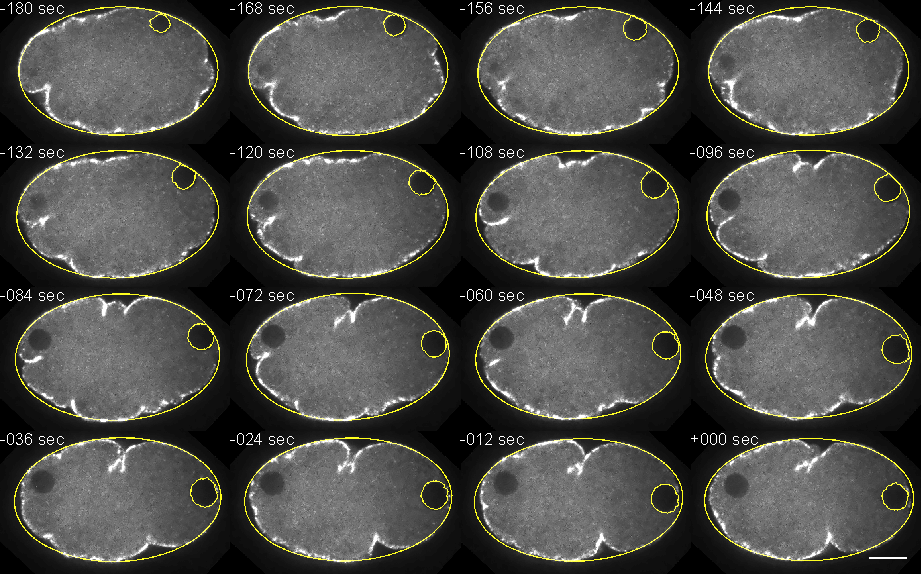
\includegraphics[width=\textwidth]{ExpMethods/FigTrackNucleus/validate.pdf}
\caption[Image analysis: Validation]{Validating the results of the segmentations, for different time-points. In each image, the outer yellow contour denotes the fitted ellipse to the segmented boundary, and the inner yellow contour denotes the segmented male pronucleus. Scale bar: \SI{10}{\unitLength}. Anterior is to the left and posterior to the right in all images. T = \SI{0}{\second} denotes end of posteriorisation.}
\label{fig:validateSegmentations}
\end{figure}

\begin{figure}[h]
\centering

\begin{subfigure}[t]{0.45\textwidth}
    \centering
    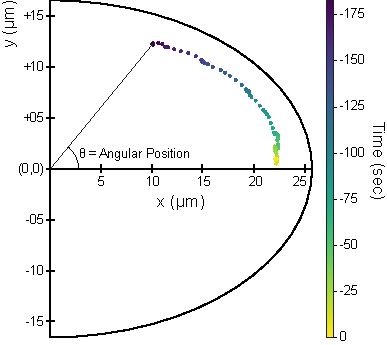
\includegraphics[width=\textwidth]{ExpMethods/FigTrackNucleus/trajectory.pdf}
    \caption{Trajectory of the male pronucleus -- denoted by the coordinates of its center -- as it posteriorises over time. Color represents time. x- and y-axes lie along the long and short axes of the ellipse fitted to the embryo boundary. Angular position is defined as the angle between the long axis and line connecting the centers of the male pronucleus and embryo.} 
    \label{subfig:malePronucleusTrackingResults-trackPronucleus}
\end{subfigure}
\hfill
\begin{subfigure}[t]{0.45\textwidth}
    \centering
    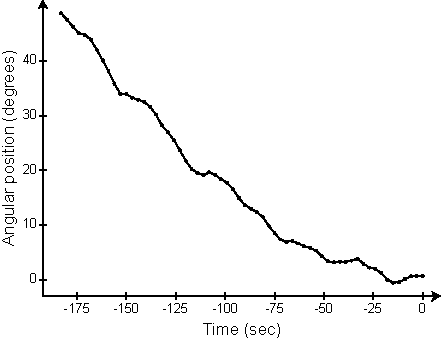
\includegraphics[width=\textwidth]{ExpMethods/FigTrackNucleus/angularPosVsTime.pdf}
    \caption{Plot of Angular position of the male pronucleus (y-axis) as a function of time (x-axis).} 
    \label{subfig:malePronucleusTrackingResults-angularPosVsTime}
\end{subfigure}

\begin{subfigure}[t]{0.45\textwidth}
    \centering
    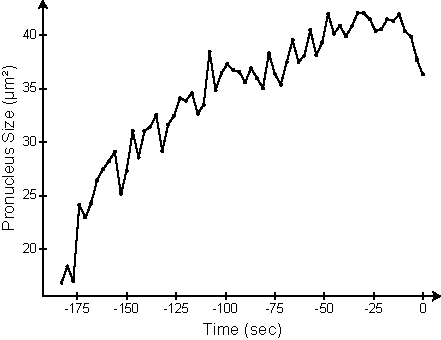
\includegraphics[width=\textwidth]{ExpMethods/FigTrackNucleus/sizeVsTime.pdf}
    \caption{Plot of the size of the male pronucleus (y-axis) as a function of time (x-axis). Size is measured as the area enclosed by the contour denoting the male pronucleus segmentation.} 
    \label{subfig:malePronucleusTrackingResults-sizeVsTime}
\end{subfigure}
\hfill
\begin{subfigure}[t]{0.45\textwidth}
    \centering
    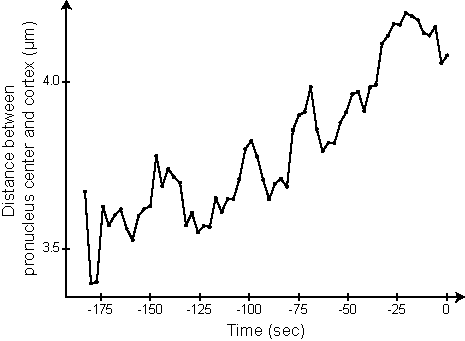
\includegraphics[width=\textwidth]{ExpMethods/FigTrackNucleus/crtxDistVsTime.pdf}
    \caption{Plot of Distance between the center of male pronucleus and closest point on cortex (y-axis) as a function of time (x-axis).} 
    \label{subfig:malePronucleusTrackingResults-crtxDistVsTime}
\end{subfigure}

\caption[Image analysis: Trajectory of male pronucleus]{Trajectory of the male pronucleus obtained using the image analysis pipeline. For all plots, T = \SI{0}{\second} denotes the end of posteriorisation. All plots are obtained from a single movie of an embryo of SWG070 strain -- same embryo depicted in \autoref{fig:imageAcquisition}, \autoref{fig:preprocess}, \autoref{fig:segmentingEmbryoBoundary}, \autoref{fig:malePronucleusTrackingPipeline} and \autoref{fig:validateSegmentations}}
\label{fig:malePronucleusTrackingResults}
\end{figure}

\begin{figure}[h]
\centering

\begin{subfigure}[t]{0.45\textwidth}
    \centering
    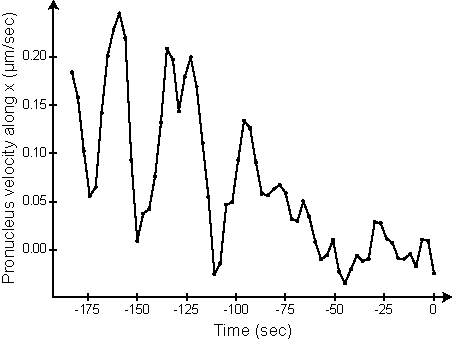
\includegraphics[width=\textwidth]{ExpMethods/FigTrackNucleus/vxVsTime.pdf}
    \caption{Plot of component of the velocity of the male pronucleus along the long axis (y-axis) as a function of time (x-axis). Positive velocity indicates movement towards posterior.} 
    \label{subfig:malePronucleusTrackingVelocities-vxVsTime}
\end{subfigure}
\hfill
\begin{subfigure}[t]{0.45\textwidth}
    \centering
    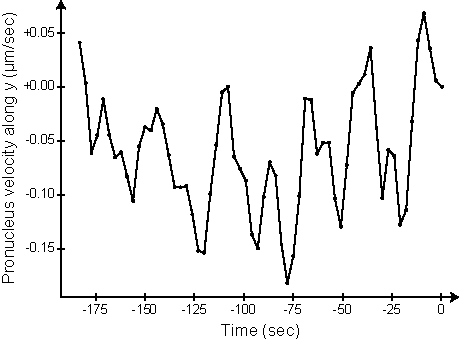
\includegraphics[width=\textwidth]{ExpMethods/FigTrackNucleus/vyVsTime.pdf}
    \caption{Plot of component of the velocity of the male pronucleus along the short axis (y-axis) as a function of time (x-axis). Positive velocity indicates movement towards the top of the embryo.} 
    \label{subfig:malePronucleusTrackingVelocities-vyVsTime}
\end{subfigure}

\begin{subfigure}[t]{0.45\textwidth}
    \centering
    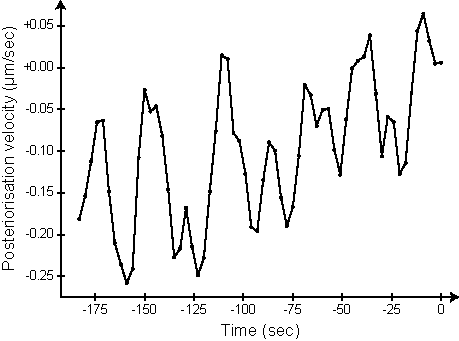
\includegraphics[width=\textwidth]{ExpMethods/FigTrackNucleus/postVelVsTime.pdf}
    \caption{Plot of the posteriorisation velocity of the male pronucleus (y-axis) as a function of time (x-axis). Posteriorisation velocity is defined as the component of the velocity of the male pronucleus parallel to the cortex. Positive velocity indicates movement towards posterior.} 
    \label{subfig:malePronucleusTrackingVelocities-postVelVsTime}
\end{subfigure}
\hfill
\begin{subfigure}[t]{0.45\textwidth}
    \centering
    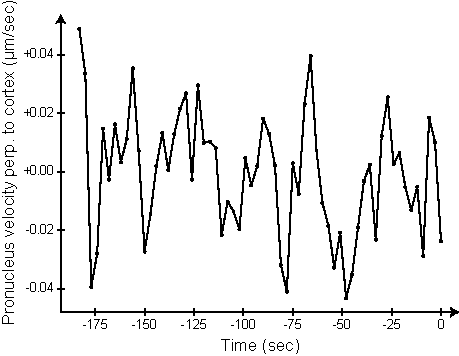
\includegraphics[width=\textwidth]{ExpMethods/FigTrackNucleus/perpVelVsTime.pdf}
    \caption{Plot of the component of the velocity of the male pronucleus perpendicular to the cortex (y-axis) as a function of time (x-axis). Positive velocity indicates movement towards the cortex.} 
    \label{subfig:malePronucleusTrackingVelocities-perpVelVsTime}
\end{subfigure}

\begin{subfigure}[t]{0.45\textwidth}
    \centering
    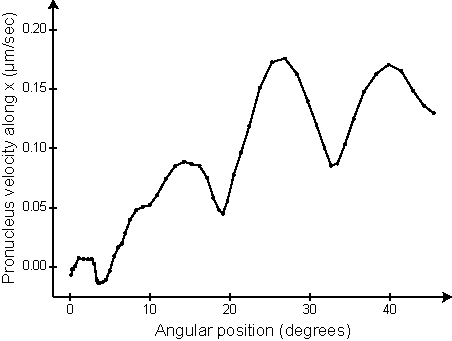
\includegraphics[width=\textwidth]{ExpMethods/FigTrackNucleus/vxVsAngleSmooth.pdf}
    \caption{Plot of component of the velocity of the male pronucleus along the long axis (y-axis) as a function of angular position (x-axis). Values have been smoothed using a sliding average with window of \num{7} frames. Positive velocity indicates movement towards posterior.} 
    \label{subfig:malePronucleusTrackingVelocities-vxVsAngleSmooth}
\end{subfigure}
\hfill
\begin{subfigure}[t]{0.45\textwidth}
    \centering
    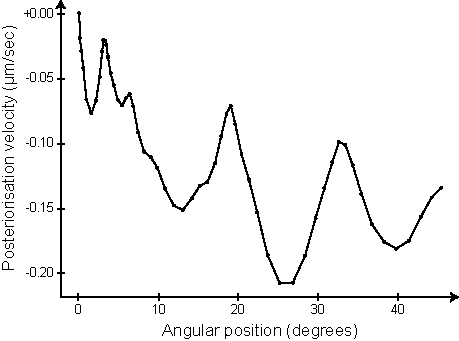
\includegraphics[width=\textwidth]{ExpMethods/FigTrackNucleus/postVelVsAngleSmooth.pdf}
    \caption{Plot of posteriorisation velocity of the male pronucleus (y-axis) as a function of angular position (x-axis). Values have been smoothed using a sliding average with window of \num{7} frames. Positive velocity indicates movement towards posterior.} 
    \label{subfig:malePronucleusTrackingVelocities-postVelVsAngleSmooth}
\end{subfigure}

\caption[Image analysis: Trajectory of male pronucleus (velocities)]{Velocities obtained using the image analysis pipeline. For plots against time, T = \SI{0}{\second} denotes the end of posteriorisation. All plots are obtained from a single movie of an embryo of SWG070 strain -- same embryo depicted in \autoref{fig:imageAcquisition}, \autoref{fig:preprocess}, \autoref{fig:segmentingEmbryoBoundary}, \autoref{fig:malePronucleusTrackingPipeline} and \autoref{fig:validateSegmentations}}
\label{fig:malePronucleusTrackingVelocities}
\end{figure}

\subsubsection{Measuring \ac{nmy2} concentrations}\label{subsubsec:myosinConc}
Myosin concentrations in the cytoplasm and cortex can be measured using the boundary segmentations and denoised myosin frames obtained from the Python script. Here we measure them in intensity per pixel units, where intensity is measured in arbitrary units corresponding to the readings from the camera used to record the movies. We consider a region \SI{15}{pixels} wide below the segmented boundary as being at the cortex, while the cytoplasm is considered as the interior region, left after the cortical region is removed. Myosin concentration in each region is estimated as the average intensity per pixel in the corresponding region, averaged over \num{7} consecutive frames (sliding window).

\subsection{Measuring cortical flows}\label{subsec:corticalFlows}
Cortical flows were measured from the denoised myosin frames using a custom \ac{matlab} script, following \cite{gross2019guiding} (\ac{matlab} script written by P. Gross). The script takes as input the boundary segmentations and the denoised myosin frames generated by the Python script, and performs two steps:
\begin{enumerate}
    \item Using the boundary segmentations already made by the Python script, the \ac{matlab} script generates a kymograph of the cortical layer in the myosin frames. The cortical layer is identified as the region starting from the boundary of the embryo and stretching \SI{30}{\pixels} deep inwards.
    \item These kymographs are then used to measure the flow velocity of the cortex as a function of position along the cortex, using \ac{piv} \citep{thielicke2014pivlab}.
\end{enumerate}
See \autoref{fig:crtxFlowMeasurement} for output kymographs and cortical flows, for the example movie considered in this chapter.

\subsubsection{Creating kymographs}\label{subsubsec:kymographs}
For a given myosin frame, its corresponding boundary segmentation (generated by the Python script) is converted into a composite B{\'e}zier curve: a series of B{\'e}zier curves joined end to end. This converts the discrete pixel positions of the boundary segmentation into a smooth curve that represents the embryo boundary. The point on this curve that is on the embryo's long axis and at the posterior end are identified. Starting from this point, additional points are sampled at one pixel size distance between adjacent points on both ends of the curve. Denoting the initial point on the posterior as zero, these points denote the integer distances along the curve, that is integer arclengths. Thus, the composite B{\'e}zier curve is used to define the distance along the cortex -- the arclength axis. 

At each point sampled on the curve, the normal to the curve pointing towards the embryo interior is found. Points are sampled along each normal at one pixel size distance between adjacent points on a normal upto a distance of \SI{30}{\pixels}, and pixel values are interpolated to obtain the estimated intensities at these points. This can be folded out into a thin rectangular \enquote{band}\footnote{The change in length between the outermost points at the boundary and innermost points towards the embryo interior are ignored, as the length of the embryo boundary is much larger than \SI{30}{\pixels}} of points along the embryo boundary. This \enquote{band} is identified as a folded out version of the cortex, calculating for the frame of interest. The long edge of this band is along the arclength axis, while the short edge is perpendicular. 

By taking the maximum intensity value along this perpendicular axis for each point on the arclength axis (maximum projection), and stacking the resultant 1D representations of myosin distributions for each frame in order of time vertically, a visualization known as the kymograph can be generated -- see \autoref{subfig:crtxFlowMeasurement-kymographFullMovie} and \autoref{subfig:crtxFlowMeasurement-kymographPosteriorization}. This kymograph allows visualization of the changes in myosin distributions as a function of time at each position on the cortex.

\subsubsection{\acf{piv}}\label{subsubsec:pivCortex}
\ac{piv} is a method of visualizing flow in fluids and measuring instantaneous flow velocities \citep{raffel1998particle,thielicke2014pivlab}. Under this method, the fluid is seeded with tracer particles which can be illuminated with light. These tracer particles are small enough that they can be assumed to faithfully follow the fluid dynamics. Time-lapse movies of the fluid flow, with the tracer particles illuminated, are taken. Instead of tracking individual particles, the flow field at a given time-point is calculated by cross-correlating sections of the frame at this time-point with the frame at the next section. In detail, the frame at the current time-point is divided into templates of defined sizes. Each template is cross-correlated with the frame at the next time-point by displacing the template upto a maximum distance from its location in the current time-point. Displacement with the largest cross-correlation, divided by the time elapsed between the two frames, is the measured velocity of the fluid at the location of the template. Here we will use a multi-pass \ac{piv} algorithm, which uses templates of different sizes to measure fluid flow at finer resolutions; along with Gaussian fitting of the peak in the cross-correlation to obtain subpixel accuracy. See \cite{raffel1998particle} for a detailed discussion. 

In the case of the cortex, since myosin motors are fluorescently labelled, tracer particles are not required -- fluorescent tags take the role of the tracer particles. To calculate cortical flow velocities along the arclength axis, the cortical \enquote{bands} extracted for each frame are used for the cross-correlations instead. A multi-pass (4 passes) PIV was utilized, with initial template size of \SI{24}{\pixels} and step size of \SI{4}{\pixels}. Max displacement of each template during cross-correlation was limited to \SI{7}{\pixels}. See \autoref{subfig:crtxFlowMeasurement-crtxFlows} for the measured cortical flows in the example movie considered for this chapter.

\begin{figure}[h]
\centering

\begin{subfigure}[t]{0.45\textwidth}
    \centering
    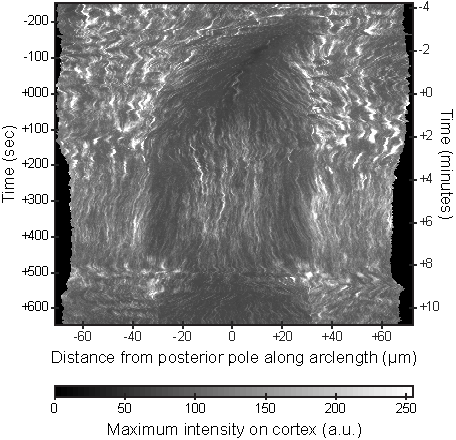
\includegraphics[width=\textwidth]{ExpMethods/FigCrtxFlows/kymographFullMovie.pdf}
    \caption{Kymograph depicting intensities along the cortex (arclength axis along x-axis) as a function of time (along y-axis), for the full movie. Colorbar indicates the maximum intensity value on the cortex at the given position and time.} 
    \label{subfig:crtxFlowMeasurement-kymographFullMovie}
\end{subfigure}
\hfill
\begin{subfigure}[t]{0.45\textwidth}
    \centering
    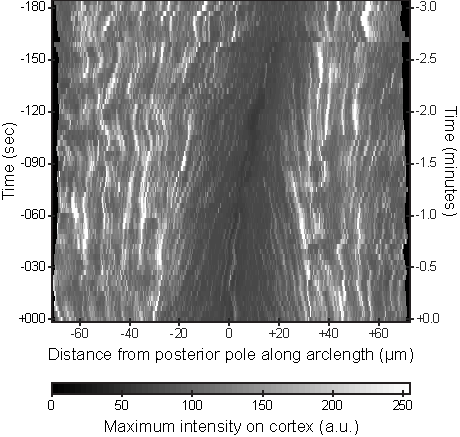
\includegraphics[width=\textwidth]{ExpMethods/FigCrtxFlows/kymographPosteriorization.pdf}
    \caption{Kymograph depicting intensities along the cortex (arclength axis along x-axis) as a function of time (along y-axis), only for time-points used to analyze posteriorisation. Colorbar indicates the maximum intensity value on the cortex at the given position and time.} 
    \label{subfig:crtxFlowMeasurement-kymographPosteriorization}
\end{subfigure}

\begin{subfigure}{\textwidth}
    \centering
    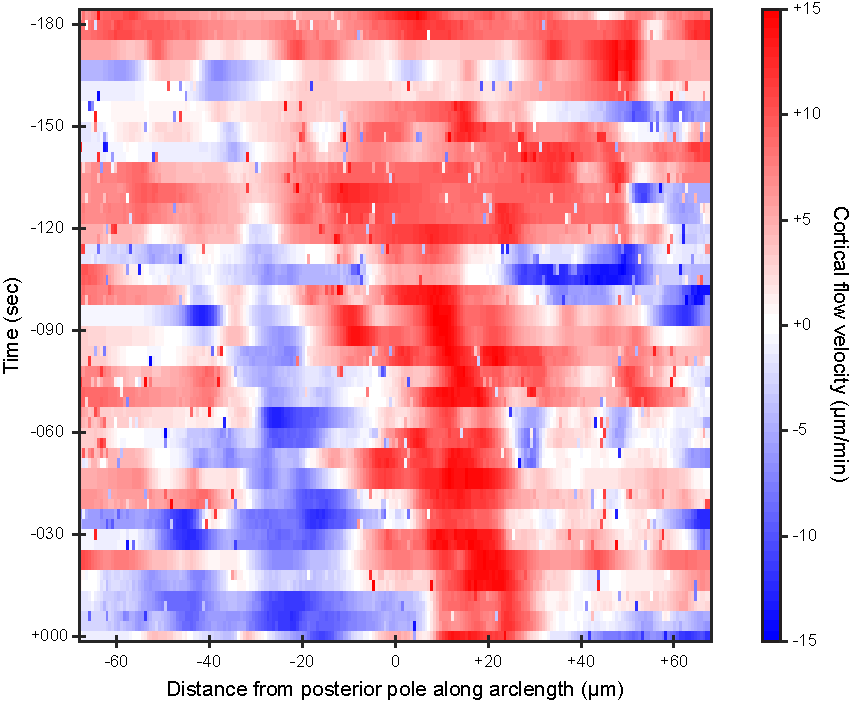
\includegraphics[width=0.8\textwidth]{ExpMethods/FigCrtxFlows/crtxFlows.pdf}
    \caption{Cortical flow velocity (colorbar) measured for the time-points used to analyse posteriorization, as a function of time (y-axis) and position along the cortex (x-axis). Positive/Negative flow velocity, depicted in red/blue, indicate movement towards/away from positive end of the arclength axis (x-axis).} 
    \label{subfig:crtxFlowMeasurement-crtxFlows}
\end{subfigure}

\caption[Image analysis: Measuring cortical flows]{Measuring cortical flows. For all plots, T = \SI{0}{\second} on the y-axis denotes the end of posteriorisation, and s = \SI{0}{\unitLength} on the x-axis denotes the posterior pole. All plots are obtained from a single movie of an embryo of SWG070 strain -- same embryo depicted in \autoref{fig:imageAcquisition}, \autoref{fig:preprocess}, \autoref{fig:segmentingEmbryoBoundary}, \autoref{fig:malePronucleusTrackingPipeline} and \autoref{fig:validateSegmentations}}
\label{fig:crtxFlowMeasurement}
\end{figure}

\subsection{Measuring cytoplasmic flows}\label{subsec:cytoFlows} %%TODO: CHECK PARAMETERS
Cytoplasmic flows in the embryos were measured using the \ac{bf} frames in the embryo movies (see \autoref{sec:imageAnalysis}). A MATLAB implementation of \ac{piv} \citep{thielicke2014pivlab} was used to calculate the flow fields in the cytoplasm from the \ac{bf} frames (see \autoref{subsec:corticalFlows} for general introduction to \ac{piv}), with the boundary segmentations (see \autoref{subsec:nucleusTracking}) used to exclude the exterior of the embryo. Yolk granules in the cytoplasm serve the role of the tracer particles in the cytoplasm. A multi-pass (4 passes) PIV was utilized, with initial template size of \SI{24}{\pixels} and step size of \SI{4}{\pixels}. Max displacement of each template during cross-correlation was limited to \SI{7}{\pixels}. 

\section{Data analysis}\label{sec:statAnalysis}
This section describes the methods used to analyse the data -- male pronucleus trajectories and cortical flows measured for each embryo -- to obtain ensemble averages for a given experiment. Primarily, we focus on average posteriorization velocity and average cortical flows as a function of angular position of the male pronucleus, for a given experimental condition. All data analysis is done using custom scripts written in \ac{matlab}.

Short-term fluctuations in each male pronucleus trajectory are smoothed using a sliding average with a window of \SI{7}{\frames} for each movie separately. To calculate average posteriorization velocity as a function of angular position, posteriorization velocity and angular positions calculated for all embryos for a given experimental condition are combined together. Angular positions in this dataset are binned in \SI{3}{\unitAngle} bins. Average posteriorization velocity for each angular position bin is calculated by averaging over all posteriorization velocities corresponding to the angular positions included in the bin. \num{95}\% confidence interval for the mean posteriorization velocities are calculated using a two-sided t-test. See \autoref{subfig:dataAnalysisExample-postVel} for an example.

Cortical flows measured for all embryos for a given experimental condition are first aligned using the arclength axis. Cortical flows are then classified using the angular position of the male pronucleus, and binned together in angular position bins of \SI{3}{\unitAngle} width each. Average cortical flows for each angular position bin are calculated by averaging all cortical flows within an angular position bin. Note that this averaging is done spatially: that is, measured flow velocities at the same position on the arclength axis corresponding to different frames are averaged together. The model described in \autoref{ch:ActiveMatter} uses these averaged cortical flows for calibration. See \autoref{subfig:dataAnalysisExample-crtxFlow} for an example.

\begin{figure}[h]
\centering

\begin{subfigure}[t]{0.45\textwidth}
    \centering
    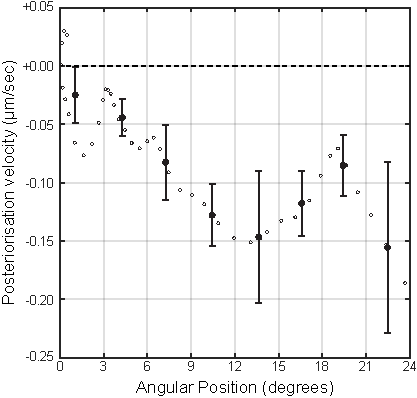
\includegraphics[width=\textwidth]{ExpMethods/FigDataAnalysis/postVel.pdf}
    \caption{Binning Posteriorization velocity (y-axis) vs Angular position (x-axis). Each angular position bin is of \SI{3}{\unitAngle} width. For each bin, the mean posteriorization velocity (dark circles) and 95\% confidence intervals of the mean (error bars) are depicted. Open circles denote the datapoints obtained after smoothing via sliding average (window: \num{7} frames). Dotted line indicates zero posteriorization velocity.} 
    \label{subfig:dataAnalysisExample-postVel}
\end{subfigure}
\hfill
\begin{subfigure}[t]{0.5\textwidth}
    \centering
    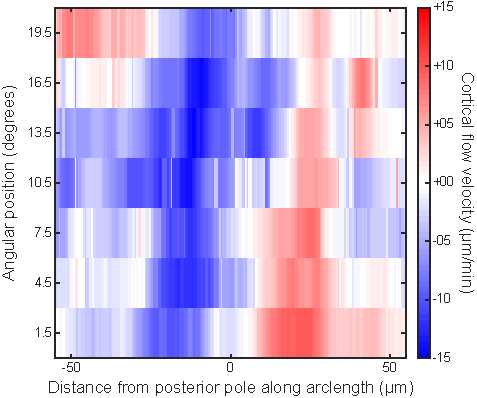
\includegraphics[width=\textwidth]{ExpMethods/FigDataAnalysis/crtxFlow.pdf}
    \caption{Binning Cortical flow velocity (colorbar) using Angular position (y-axis). Each angular position bin is of \SI{3}{\unitAngle} width. For each bin, the mean cortical flow at each position along the cortex (x-axis) is calculated -- using all frames that fall within the angular position bin. Positive/Negative flow velocity, depicted in red/blue, indicate movement towards/away from positive end of the arclength axis (x-axis). s = \SI{0}{\unitLength} on the x-axis denotes the posterior pole.} 
    \label{subfig:dataAnalysisExample-crtxFlow}
\end{subfigure}

\caption[Data Analysis (example movie only)]{Data analysis done for a single movie of an embryo of SWG070 strain -- depicted in \autoref{fig:imageAcquisition}, \autoref{fig:preprocess}, \autoref{fig:segmentingEmbryoBoundary}, \autoref{fig:malePronucleusTrackingPipeline} and \autoref{fig:validateSegmentations}. This figure showcases the two main output graphs we obtain from our data analysis.}
\label{fig:dataAnalysisExample}
\end{figure}